% !TeX program = xelatex
% !TeX encoding = UTF-8
% Compile from the project root; ATT48 figures and experiment records are bundled.
% Compile twice: xelatex tsp_simulated_annealing.tex
\documentclass[UTF8,a4paper,11pt,fontset=none]{ctexart}

% ---------- Page layout and typography ----------
\usepackage[margin=24mm,top=23mm,bottom=24mm,headheight=16pt,headsep=8mm]{geometry}
\usepackage{fontspec}
\setCJKmainfont{FandolSong-Regular}[Extension=.otf,Script=Default,
  BoldFont=FandolSong-Bold,ItalicFont=FandolKai-Regular]
\setCJKsansfont{FandolHei-Regular}[Extension=.otf,Script=Default,
  BoldFont=FandolHei-Bold]
\setCJKmonofont{FandolSong-Regular}[Extension=.otf,Script=Default]
\usepackage{amsmath}
\usepackage{unicode-math}
\setmainfont{TeX Gyre Pagella}
\setsansfont{TeX Gyre Heros}
\setmonofont{TeX Gyre Cursor}[Scale=MatchLowercase]
\setmathfont{TeX Gyre Pagella Math}
\usepackage{xcolor}
\definecolor{accent}{HTML}{234E70}
\definecolor{muted}{HTML}{586574}
\definecolor{pale}{HTML}{F3F6F8}
\usepackage{setspace}
\setstretch{1.23}
\setlength{\parindent}{2em}
\setlength{\parskip}{0.2em}
\setlength{\emergencystretch}{2em}
\raggedbottom
\clubpenalty=10000
\widowpenalty=10000
\displaywidowpenalty=10000
\usepackage{needspace}
\ctexset{
  section={format=\Large\sffamily\bfseries\color{accent},
    beforeskip=1.3ex plus .3ex,afterskip=.8ex},
  subsection={format=\large\sffamily\bfseries,
    beforeskip=1.2ex plus .3ex,afterskip=.5ex},
  subsubsection={format=\normalsize\sffamily\bfseries,
    beforeskip=1ex,afterskip=.4ex}
}
\usepackage{fancyhdr}
\pagestyle{fancy}
\fancyhf{}
\fancyhead[L]{\small\sffamily\color{muted}经典 TSP 问题的模拟退火算法}
\fancyhead[R]{\small\sffamily\color{muted}模型 · 原理 · 实现}
\fancyfoot[C]{\small\thepage}
\renewcommand{\headrulewidth}{0.3pt}

% ---------- Lists, tables, illustrations and algorithms ----------
\usepackage{enumitem}
\setlist{topsep=3pt,itemsep=2pt,parsep=0pt,leftmargin=2em}
\usepackage{booktabs,tabularx,array}
\usepackage{graphicx}
\renewcommand{\arraystretch}{1.2}
\usepackage[font=small,labelfont=bf,labelsep=quad]{caption}
\usepackage{tikz}
\usetikzlibrary{arrows.meta}
\usepackage[most]{tcolorbox}
\newtcolorbox{keypoint}[1]{
  enhanced,breakable,colback=pale,colframe=accent,
  boxrule=0pt,leftrule=2pt,arc=0pt,
  left=9pt,right=9pt,top=7pt,bottom=7pt,
  before skip=8pt,after skip=8pt,
  title={#1},colbacktitle=pale,coltitle=accent,
  fonttitle=\sffamily\bfseries,attach title to upper={\quad}
}
\usepackage[ruled,vlined,linesnumbered]{algorithm2e}
\SetAlgorithmName{算法}{算法}{算法目录}
\SetKwInput{KwIn}{输入}
\SetKwInput{KwOut}{输出}
\SetKw{Return}{返回}
\SetKwFor{While}{当}{时}{结束循环}
\SetKwFor{For}{对}{执行}{结束循环}
\SetKwIF{If}{ElseIf}{Else}{若}{则}{否则若}{否则}{结束判断}
\DontPrintSemicolon
\SetAlFnt{\small\setstretch{1.1}}
\SetAlCapFnt{\small\bfseries}
\SetAlCapNameFnt{\small\bfseries}
\SetAlgoNlRelativeSize{-1}
\SetAlgoInsideSkip{smallskip}
\usepackage{listings}
\lstset{
  basicstyle=\ttfamily\small,keywordstyle=\color{accent}\bfseries,
  commentstyle=\color{muted},stringstyle=\color{accent},
  backgroundcolor=\color{pale},frame=none,
  columns=fullflexible,keepspaces=true,showstringspaces=false,
  breaklines=true,tabsize=4,xleftmargin=8pt,xrightmargin=8pt,
  aboveskip=8pt,belowskip=8pt
}

% ---------- Mathematics and references ----------
\numberwithin{equation}{section}
\newcommand{\states}{\mathcal{S}}
\newcommand{\best}{\mathrm{best}}
\newcommand{\bigO}{\mathcal{O}}
\DeclareMathOperator{\Unif}{Unif}
\DeclareMathOperator*{\argmin}{arg\,min}
\usepackage{hyperref}
\hypersetup{
  unicode=true,colorlinks=true,linkcolor=accent,citecolor=accent,urlcolor=accent,
  pdftitle={经典 TSP 问题的模拟退火算法},
  pdfsubject={对称旅行商问题、Metropolis 接受准则与 2-opt 邻域},
  pdfauthor={},bookmarksnumbered=true
}
\usepackage[nameinlink,noabbrev]{cleveref}
\crefname{equation}{式}{式}
\crefname{figure}{图}{图}
\crefname{table}{表}{表}
\crefname{algocf}{算法}{算法}

\begin{document}
\thispagestyle{plain}
\begin{center}
  {\small\sffamily\color{accent}组合优化\quad / \quad 算法讲义}\par
  \vspace{7pt}
  {\LARGE\sffamily\bfseries 经典 TSP 问题的模拟退火算法}\par
  \vspace{5pt}
  {\normalsize\color{muted}问题建模、数学原理与可执行算法}\par
\end{center}
\vspace{2pt}
\noindent{\color{accent}\rule{\linewidth}{0.7pt}}
\vspace{3pt}

\noindent\textbf{摘要}\quad
本文以完全图上的对称旅行商问题为对象，给出排列形式的数学模型，解释模拟退火的
Boltzmann 分布与 Metropolis 接受准则，并详细推导基于 2-opt 区间反转的求解算法。
文中包含温度设置、完整伪代码、手算示例、复杂度分析及已验证的 Python 实现使用方法，
并给出 C++17 对美国本土 48 州首府经典实例 ATT48 的求解、逐提案可视化、地理地图与收敛实验。
模拟退火用于在有限计算预算内寻找高质量路线，其输出一般不附带全局最优性证明。

\vspace{4pt}
\noindent\textbf{关键词}\quad 旅行商问题；模拟退火；Metropolis 准则；2-opt；组合优化
\vspace{7pt}

\section{经典 TSP 问题}
\subsection{问题定义与基本假设}
旅行商问题（Traveling Salesman Problem，TSP）要求：给定一组城市以及任意两城市之间的
旅行费用，从一个城市出发，访问其余每个城市恰好一次，最后返回出发城市，使总费用最小
\cite{waterloo}。费用可以是距离、时间或其他固定成本。

本文研究一名旅行商、无容量与时间窗等附加约束的情形。城市集合与距离矩阵记为
\begin{equation}
  V=\{0,1,\ldots,n-1\},\qquad D=(d_{ij})_{n\times n},\qquad n\geq3.
\end{equation}
任意城市对之间均存在有限费用。对称 TSP 满足
\begin{equation}
  d_{ij}=d_{ji}\geq0,\qquad d_{ii}=0.
  \label{eq:symmetry}
\end{equation}
若城市具有二维坐标 $(x_i,y_i)$，可取欧氏距离
\begin{equation}
  d_{ij}=\sqrt{(x_i-x_j)^2+(y_i-y_j)^2}.
\end{equation}
一般的对称 TSP 不要求距离来自坐标，也不必满足三角不等式。
下面的四边增量公式依赖的是\textbf{距离对称性}。

\subsection{解的表示与优化目标}
固定城市 $0$ 为起点，用城市排列表示路线：
\begin{equation}
  s=(v_0,v_1,\ldots,v_{n-1}),\qquad v_0=0,\qquad v_n=v_0.
\end{equation}
设 $\states$ 为所有此类排列的集合，则闭环长度及优化目标为
\begin{align}
  C(s)&=\sum_{k=0}^{n-1}d_{v_k,v_{k+1}},
  \label{eq:cost}\\
  C^\star&=\min_{s\in\states}C(s),\qquad
  s^\star\in\argmin_{s\in\states}C(s).
  \label{eq:objective}
\end{align}
排列保证每个城市恰好出现一次，最后一项 $d_{v_{n-1},v_0}$ 保证返回起点。
例如，排列 $(0,2,1,3)$ 对应回路 $0\to2\to1\to3\to0$。
图论上，目标是在加权完全图中寻找最短哈密顿回路。

\subsection{问题规模与启发式求解}
固定起点只消除了循环移位的重复表示，不会遗漏任何回路。
若再将正向与反向视为同一条无向回路，则不同回路的数量为
\begin{equation}
  \frac{(n-1)!}{2}.
\end{equation}
候选数量呈阶乘增长。TSP 的优化版本是 NP-hard；相应的标准判定版本是
NP-complete\cite{cook}。模拟退火通过随机邻域搜索减少实际考察的路线数量，
以计算预算换取解的质量，但不保证有限时间内一定找到全局最优路线。

\section{模拟退火的数学原理}
\subsection{从退火过程到概率分布}
模拟退火（Simulated Annealing，SA）借鉴物理退火：把目标函数值视为系统能量，
将温度 $T>0$ 作为控制随机性的参数，逐渐降温以偏向低成本状态\cite{kirkpatrick}。
固定温度下，考虑 Boltzmann 分布
\begin{equation}
  \pi_T(s)=\frac{\exp[-C(s)/T]}{Z(T)},\qquad
  Z(T)=\sum_{u\in\states}\exp[-C(u)/T].
  \label{eq:boltzmann}
\end{equation}
目标值越低，状态的概率越大。有限状态空间上，当 $T\to0^+$ 时，该分布的概率质量
集中到全局最优解集合。这里已将物理中的 Boltzmann 常数吸收到温度中，
因此 $T$ 应与路线费用使用相同的尺度。

\subsection{Metropolis 接受准则}
从当前路线 $s$ 产生候选路线 $s'$，定义成本差
\begin{equation}
  \Delta=C(s')-C(s).
  \label{eq:delta}
\end{equation}
如果候选生成概率对称，即 $q(s'\mid s)=q(s\mid s')$，则接受概率为
\begin{equation}
  \boxed{
  A_T(s,s')=\min\{1,\exp(-\Delta/T)\}
  =\begin{cases}
    1, & \Delta\leq0,\\[2pt]
    \exp(-\Delta/T), & \Delta>0.
  \end{cases}}
  \label{eq:metropolis}
\end{equation}
这就是 Metropolis 准则\cite{metropolis}：改善或等长的候选直接接受，变差的候选按概率接受。
指数形式对应于
\begin{equation}
  \frac{\pi_T(s')}{\pi_T(s)}
  =\exp\!\left[-\frac{C(s')-C(s)}{T}\right]
  =\exp(-\Delta/T).
\end{equation}
归一化常数 $Z(T)$ 被约去，算法不必枚举全部路线。

设 $P_T$ 是包含接受与拒绝操作的转移概率。
对称提案与\cref{eq:metropolis}使其满足细致平衡：
\begin{equation}
  \pi_T(s)P_T(s,s')=\pi_T(s')P_T(s',s).
\end{equation}
因此 $\pi_T$ 是固定温度链的平稳分布；在连通性、非周期性等相应条件下，
足够多的转移可趋近该分布。有限次搜索并不意味着已经达到平衡。
如果提案概率不对称，应改用包含反向与正向提案概率比的
Metropolis--Hastings 接受率：
\begin{equation}
  A_T(s,s')=\min\!\left\{1,
    \exp(-\Delta/T)\frac{q(s\mid s')}{q(s'\mid s)}\right\}.
\end{equation}

\subsection{接受变差与逐步降温}
只接受改善的搜索可能停在局部最优。接受暂时变差的路线，使算法有机会穿过高成本区域，
进入更好的搜索区域。以 $\Delta=10$ 为例：
\begin{equation*}
  \begin{aligned}
    T=100&:\quad \exp(-10/100)\approx0.9048,\\
    T=10&:\quad \exp(-10/10)\approx0.3679,\\
    T=1&:\quad \exp(-10)\approx4.54\times10^{-5}.
  \end{aligned}
\end{equation*}
高温时探索较充分，低温时主要接受改善。工程中常用几何降温：
\begin{equation}
  T_{k+1}=\alpha T_k,\qquad 0<\alpha<1.
  \label{eq:cooling}
\end{equation}
在适当条件下，足够慢的对数降温 $T_t=c/\ln(1+t)$ 可使状态依概率趋向全局最优集合，
其中 $c$ 需满足与能垒深度有关的条件\cite{hajek}。

\begin{keypoint}{理论结论的适用范围}
固定温度的平稳分布、无限时间下的渐近收敛、有限轮次的实际输出是不同层次的结论。
本文采用的几何降温和有限计算预算\textbf{不构成全局最优性保证}。
\end{keypoint}

\section{面向 TSP 的模拟退火算法}
\subsection{初始化与状态保存}
先构造距离矩阵，固定 $v_0=0$，随机打乱其余城市，得到初始路线 $s$。
也可采用最近邻法构造初始路线。然后计算完整闭环长度，并初始化
\begin{equation}
  C\gets C(s),\qquad s_{\best}\gets s,\qquad C_{\best}\gets C(s).
\end{equation}
其中 $s$ 是当前路线，$s_{\best}$ 是历史最好路线。
\textbf{当前路线允许变差，历史最好路线只在找到更优结果时更新。}
程序保存最好路线时须复制列表，避免后续原地修改影响已保存的结果。

\subsection{邻域设计：2-opt 区间反转}
均匀选取两个不同位置 $1\leq i<j\leq n-1$，将子序列 $(v_i,\ldots,v_j)$ 反转。
例如，反转城市 $B,C,D$ 对应的区间：
\begin{equation*}
  \begin{aligned}
    s &: 0\to A\to B\to C\to D\to E\to0,\\
    s'&: 0\to A\to D\to C\to B\to E\to0.
  \end{aligned}
\end{equation*}
该操作始终保持城市排列的合法性及回路的连通性，无须引入约束罚函数。
同一区间反转两次即可恢复原路线，且位置对的选择概率与路线无关，故提案对称。
相邻位置的反转就是相邻交换，所以该邻域能连接全部固定起点的排列。

实现中也允许反转全部非起点城市。它仅改变整个无向回路的方向，成本不变，
是无害但没有改进作用的提案。

\subsection{四边增量公式及其推导}
记区间的边界城市为
\begin{equation}
  a=v_{i-1},\qquad b=v_i,\qquad c=v_j,\qquad
  d=v_{(j+1)\bmod n}.
\end{equation}
原边界上的 $(a,b)$、$(c,d)$ 被替换为 $(a,c)$、$(b,d)$。
由距离对称性，区间内部的边虽然反向，但费用不变。因此
\begin{equation}
  \boxed{\Delta=d_{ac}+d_{bd}-d_{ab}-d_{cd}.}
  \label{eq:twoopt}
\end{equation}
只读取四个矩阵元素，就能以 $\bigO(1)$ 时间评价候选。
当 $j=n-1$ 时，$d=v_0$，该公式也正确包含返回起点的边。

非对称 TSP 中，内部边的反向成本也会变化，完整增量应为
\begin{equation}
  \Delta_{\mathrm{asym}}
  =d_{ac}+d_{bd}-d_{ab}-d_{cd}
   +\sum_{k=i}^{j-1}\bigl(d_{v_{k+1},v_k}-d_{v_k,v_{k+1}}\bigr).
\end{equation}
因此不能把\cref{eq:twoopt}直接用于非对称矩阵；配套程序会拒绝此类输入。

\subsection{接受操作与最好解更新}
\begin{enumerate}[label=\arabic*.]
  \item 若 $\Delta\leq0$，接受候选路线。
  \item 若 $\Delta>0$，生成 $u\sim\Unif([0,1))$；当 $u<\exp(-\Delta/T)$ 时接受。
  \item 接受时，实际反转区间并令 $C\gets C+\Delta$；拒绝时，当前路线保持不变。
  \item 若更新后的 $C<C_{\best}$，复制当前路线并更新历史最好长度。
\end{enumerate}
\textbf{接受概率中的差值必须相对于当前解计算，不能相对于历史最好解计算。}

\subsection{温度标定、搜索长度与停止条件}
\textbf{初始温度。}
在初始路线处试采样若干 2-opt 提案，将正增量的均值记为 $\overline{\Delta_+}$。
若希望这一典型变差量的初始接受概率为 $p_0\in(0,1)$，则
\begin{equation}
  p_0=\exp\!\left(-\frac{\overline{\Delta_+}}{T_0}\right)
  \quad\Longrightarrow\quad
  \boxed{T_0=-\frac{\overline{\Delta_+}}{\ln p_0}.}
  \label{eq:tzero}
\end{equation}
这只标定平均变差量对应的接受概率，不意味着所有变差提案的平均接受率恰好为 $p_0$。
示例试采样 200 次，取 $p_0=0.8$；若未采到正增量，则使用最大边权作为初温，
全部边权为零时使用 $T_0=1$。

\textbf{同温度搜索与降温。}
在每个温度执行 $L$ 次提案，包括被拒绝的提案，然后按\cref{eq:cooling}降温。
$L$ 是搜索预算，不是已经达到平衡的保证。$\alpha$ 越接近 1，覆盖同一温度范围所需的层数越多。

\textbf{停止条件。}
当 $T\leq T_{\min}$ 或温度层数达到 $K_{\max}$ 时停止。
采用 $T_{\min}=10^{-4}T_0$ 有助于适应距离单位的整体缩放。
还可以设置总运行时间上限，或多次独立重启后选取最好的结果。

\begin{table}[htbp]
  \centering
  \caption{配套实现的教学参数；这些取值并非普适最优设置}
  \label{tab:parameters}
  \small
  \begin{tabularx}{\linewidth}{@{}lclX@{}}
    \toprule
    参数 & 符号 & 示例取值 & 作用 \\
    \midrule
    典型变差接受率 & $p_0$ & $0.8$ & 标定初温的费用尺度 \\
    降温系数 & $\alpha$ & $0.98$ & 控制温度下降速度 \\
    每层提案次数 & $L$ & $100n$ & 控制同温度搜索预算 \\
    相对终温 & $T_{\min}/T_0$ & $10^{-4}$ & 设置温度停止阈值 \\
    最大温度层数 & $K_{\max}$ & $2000$ & 限制总搜索层数 \\
    \bottomrule
  \end{tabularx}
\end{table}

\subsection{完整算法}
算法~\ref{alg:sa} 用精确算术描述主流程。实际实现会在每层结束及准备保存新纪录时，
重算完整路线长度，以减轻浮点增量的累积误差。

\begin{algorithm}[htbp]
  \caption{基于 2-opt 的对称 TSP 模拟退火算法}
  \label{alg:sa}
  \KwIn{对称距离矩阵 $D$；$T_0>T_{\min}>0$；$0<\alpha<1$；
    每层提案次数 $L$；最大层数 $K_{\max}$。}
  \KwOut{搜索过程中发现的最好路线 $s_{\best}$ 及其长度 $C_{\best}$。}
  固定起点 $v_0=0$，随机排列其余城市，得到 $s$\;
  $C\gets\sum_{r=0}^{n-1}d_{v_r,v_{(r+1)\bmod n}}$\;
  $s_{\best}\gets\operatorname{copy}(s)$，$C_{\best}\gets C$\;
  $T\gets T_0$，$k\gets0$\;
  \While{$T>T_{\min}$ 且 $k<K_{\max}$}{
    \For{$\ell=1,2,\ldots,L$}{
      均匀选择位置对 $1\leq i<j\leq n-1$\;
      $a\gets v_{i-1}$，$b\gets v_i$，$c\gets v_j$，$d\gets v_{(j+1)\bmod n}$\;
      $\Delta\gets d_{ac}+d_{bd}-d_{ab}-d_{cd}$\;
      生成 $u\sim\Unif([0,1))$\;
      \If{$\Delta\leq0$ 或 $u<\exp(-\Delta/T)$}{
        反转 $s$ 的第 $i$ 至第 $j$ 个位置\;
        $C\gets C+\Delta$\;
        \If{$C<C_{\best}$}{
          $s_{\best}\gets\operatorname{copy}(s)$，$C_{\best}\gets C$\;
        }
      }
    }
    $T\gets\alpha T$，$k\gets k+1$\;
  }
  \Return{$(s_{\best},C_{\best})$}\;
\end{algorithm}

\Needspace{10\baselineskip}
\subsection{时间与空间复杂度}
设实际执行 $K$ 个温度层，每层提出 $L$ 次候选：
\begin{itemize}
  \item 距离矩阵的构造与存储分别需要 $\bigO(n^2)$ 时间和空间。
  \item 四边增量评价需要 $\bigO(1)$ 时间，全部评价共需 $\bigO(KL)$ 时间。
  \item Python 列表的区间反转最坏为 $\bigO(n)$；复制最好路线也是 $\bigO(n)$。
\end{itemize}
所以本实现的最坏总时间与总空间分别为
\begin{equation}
  \boxed{\text{时间：}\ \bigO(n^2+KLn),\qquad
  \text{空间：}\ \bigO(n^2).}
\end{equation}
矩阵之外的工作空间为 $\bigO(n)$。不能把 $\bigO(1)$ 的增量评价误认为整个提案更新都是常数时间。
无最大层数限制且 $T_0>T_{\min}$ 时，几何降温所需的层数为
\begin{equation}
  K=\left\lceil\frac{\ln(T_{\min}/T_0)}{\ln\alpha}\right\rceil.
\end{equation}
当 $T_{\min}/T_0=10^{-4}$、$\alpha=0.98$ 时，需执行 456 个温度层。

\section{示例与实现验证}
\subsection{四城市手算示例}
取单位正方形的顶点为城市坐标，以 $\symbfit{x}_r$ 表示城市 $r$ 的坐标：
\begin{equation*}
  \symbfit{x}_0=(0,0),\quad \symbfit{x}_1=(1,0),\quad
  \symbfit{x}_2=(1,1),\quad \symbfit{x}_3=(0,1).
\end{equation*}
当前路线为 $0\to2\to1\to3\to0$。反转位置 1 至 2，得到
$0\to1\to2\to3\to0$，如\cref{fig:twoopt}所示。

\begin{figure}[htbp]
  \centering
  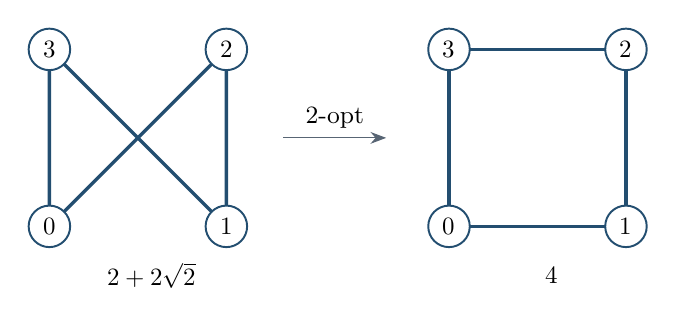
\begin{tikzpicture}[scale=1.45,
    city/.style={circle,fill=white,draw=accent,line width=.7pt,
      inner sep=2pt,minimum size=15pt,font=\small},
    tour/.style={draw=accent,line width=1.2pt}]
    \begin{scope}
      \draw[tour] (0,0)--(1.55,1.55)--(1.55,0)--(0,1.55)--cycle;
      \node[city] at (0,0) {$0$};
      \node[city] at (1.55,0) {$1$};
      \node[city] at (1.55,1.55) {$2$};
      \node[city] at (0,1.55) {$3$};
      \node[font=\small] at (.775,-.43) {反转前：$2+2\sqrt2$};
    \end{scope}
    \draw[-{Stealth[length=2mm]},draw=muted] (2.05,.775)--(2.95,.775)
      node[midway,above,font=\small] {2-opt};
    \begin{scope}[xshift=3.5cm]
      \draw[tour] (0,0)--(1.55,0)--(1.55,1.55)--(0,1.55)--cycle;
      \node[city] at (0,0) {$0$};
      \node[city] at (1.55,0) {$1$};
      \node[city] at (1.55,1.55) {$2$};
      \node[city] at (0,1.55) {$3$};
      \node[font=\small] at (.775,-.43) {反转后：$4$};
    \end{scope}
  \end{tikzpicture}
  \caption{单位正方形上的一次 2-opt 更新。节点为城市编号，线段为无向路线；每条正方形边的长度为 1。}
  \label{fig:twoopt}
\end{figure}

依据\cref{eq:twoopt}，差值为
\begin{equation}
  \begin{aligned}
    \Delta
    &=d_{0,1}+d_{2,3}-d_{0,2}-d_{1,3}\\
    &=2-2\sqrt2\approx-0.828427.
  \end{aligned}
\end{equation}
由于 $\Delta<0$，该更新必然接受，新长度为 4。
反向操作的增量为 $+0.828427$，则是否接受由当前温度决定。

\Needspace{13\baselineskip}
\subsection{Python 实现与可复现实验}
配套文件 \texttt{tsp\_sa.py} 仅使用 Python 标准库。
\texttt{test\_tsp\_sa.py} 包含验证程序。在项目目录执行：
\begin{lstlisting}[language=bash]
python tsp_sa.py
python -m unittest -v
\end{lstlisting}
\Needspace{11\baselineskip}
也可以用自己的坐标调用：
\begin{lstlisting}[language=Python]
from tsp_sa import euclidean_distances, simulated_annealing_tsp

points = [(0, 0), (1, 0), (1, 1), (0, 1)]
distance = euclidean_distances(points)
result = simulated_annealing_tsp(distance, seed=42)

print(result.route + [result.route[0]])
print(result.length)
\end{lstlisting}
返回的 \texttt{route} 仅保存每个城市一次，\texttt{length} 已包含返回起点的距离。
程序还支持直接输入有限、非负、严格对称且对角线为零的距离矩阵。

\Needspace{8\baselineskip}
十城市合成示例使用以下坐标，距离单位仅用于教学：
\begin{equation*}
  \begin{aligned}
    &(0,0),\ (2,1),\ (4,0),\ (6,2),\ (5,5),\\
    &(3,6),\ (1,5),\ (-1,3),\ (2,3),\ (4,3).
  \end{aligned}
\end{equation*}
在 Python 3.13.5、随机种子 42 及\cref{tab:parameters}参数下，实测结果为
\begin{equation*}
  \begin{aligned}
    C_{\mathrm{initial}}&=41.146372,&
    C_{\best}&=24.643181,\\
    T_0&=9.609163,&
    K&=456.
  \end{aligned}
\end{equation*}
共提出 456\,000 次候选，接受 83\,142 次；最好路线为
\begin{equation*}
  0\to7\to8\to6\to5\to4\to9\to3\to2\to1\to0.
\end{equation*}
该运行只报告搜索到的最好路线，不提供该十城市实例的最优性证明。

五项自动验证全部通过：四边增量与完整重算一致；七城市实例的三个指定种子均达到穷举最优值；
固定种子可复现且距离缩放检查通过；零距离、三城市及迭代上限处理正确；非对称输入被拒绝。
这些是针对具体实例和实现行为的验证，不能推广为模拟退火的普遍最优性保证。

\clearpage
% Reproducible experiment; numerical macros are generated from C++ output.
% Generated by scripts/make_figures.py
\newcommand{\AttBest}{10628}
\newcommand{\AttInitial}{49454}
\newcommand{\AttTemperature}{2522.862044}
\newcommand{\AttProposals}{2\,188\,800}
\newcommand{\AttAccepted}{346\,966}
\newcommand{\AttFirstBest}{1\,076\,288}
\newcommand{\AttMean}{10687.70}
\newcommand{\AttMedian}{10673.00}
\newcommand{\AttStd}{54.55}
\newcommand{\AttWorst}{10840}
\newcommand{\AttHits}{3}
\newcommand{\AttMeanGap}{0.562}
\newcommand{\AttReduction}{78.51}
\newcommand{\AttMeanTime}{0.0726}

\section{经典实例实验：美国本土 48 州首府}
\subsection{数据来源、地图与距离定义}
选用 TSPLIB 的 \texttt{att48} 实例。官方文件说明为“48 capitals of the US
(Padberg/Rinaldi)”，含 48 个城市，类型为对称 TSP，边权类型为
\texttt{ATT}\cite{tsplib}。它对应美国本土相连 48 州的首府，不含阿拉斯加、
夏威夷及华盛顿特区。固定起点并去除反向重复后有 $47!/2$ 条不同回路，
适合在普通计算机上观察启发式搜索。

原始文件 \texttt{data/att48.tsp} 与参考路线 \texttt{data/att48.opt.tour}
均从海德堡大学 TSPLIB 官方站点获取。官方公布的最优费用为
$C^\star=10628$\cite{attbest}。参考路线仅用于独立验证，\textbf{不参与初始化、
搜索或停止判断}。本节在输入输出中使用 TSPLIB 的 $1,\ldots,48$ 编号，
C++ 内部仍使用从 0 开始的下标。

ATT 坐标不是经纬度；按 TSPLIB 定义，令
\begin{equation}
 r_{ij}=\sqrt{\frac{(x_i-x_j)^2+(y_i-y_j)^2}{10}},\quad
 t_{ij}=\left\lfloor r_{ij}+\frac12\right\rfloor,\quad
 d_{ij}=\begin{cases}t_{ij}+1,&t_{ij}<r_{ij},\\t_{ij},&t_{ij}\geq r_{ij}.\end{cases}
 \label{eq:att-distance}
\end{equation}
因此总费用是整数 ATT 单位，不能解释为公里或实际公路里程。
地理图采用 Natural Earth 的州界和首府位置\cite{naturalearth}；按照州名的
英文字母顺序，将本土 48 州的首府与实例编号对应。经纬度只用于地图展示，
所有优化及费用计算均使用原始坐标和\cref{eq:att-distance}。

\begin{figure}[htbp]
 \centering
 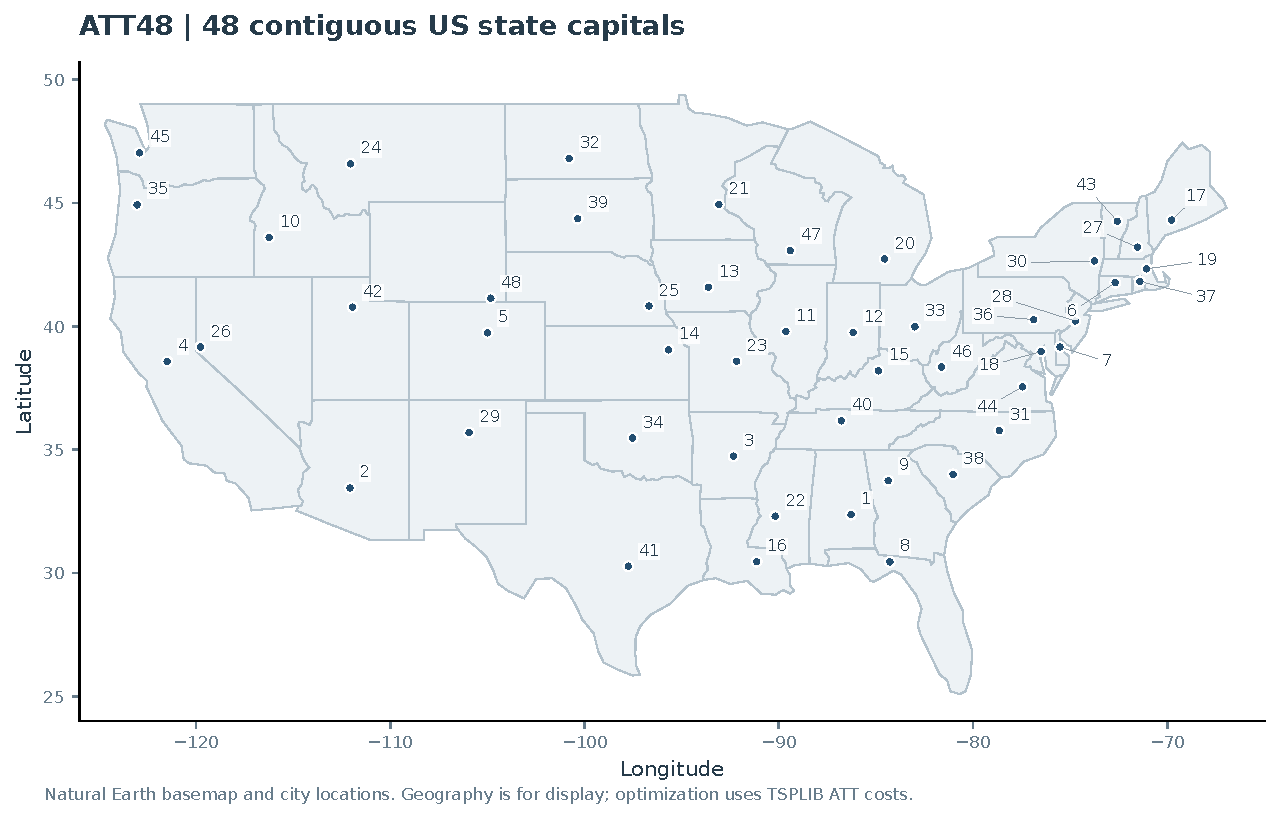
\includegraphics[width=.98\linewidth]{figures/att48_map.pdf}
 \caption{ATT48 对应的美国本土 48 州首府地理示意图。数字为 TSPLIB 节点编号；
 州界为概化底图。完整编号、州名、首府与经纬度见 \texttt{data/att48\_capitals.csv}。}
 \label{fig:att-map}
\end{figure}

\clearpage
\subsection{C++ 实现与每一步搜索的可视化}
\texttt{src/tsp.hpp} 实现数据解析、整数距离矩阵、初温采样和模拟退火；
\texttt{src/main.cpp} 处理用户选项并导出实验记录；
\texttt{src/visualizer.hpp} 使用 Windows 原生 GDI 窗口绘制路线。
求解器采用 C++17，不依赖第三方图形库；无界面求解也可在其他支持 C++17 的系统编译。
Python 仅用于实验后的绘图，不承担本节 TSP 求解。

算法沿用前文的随机初始排列、200 次初温试采样、2-opt 提案、Metropolis 接受准则、
几何降温与历史最好解保存。使用 64 位整数保存边权及路径费用，避免 ATT 费用累积误差。
核心循环中的更新和可视化调用如下（省略外围变量定义）：
\begin{lstlisting}[language=C++]
const auto [i, j] = rng.pair(n);
const Cost change = delta(route, p.distance, i, j);
const bool accept = change <= 0 ||
    rng.uniform() < std::exp(-double(change) / temperature);
++out.proposals;
if (accept) {
    std::reverse(route.begin()+i, route.begin()+j+1);
    current += change;
    ++out.accepted;
    if (current < out.best) {
        out.best = current;
        out.route = route;
        out.best_iteration = out.proposals;
    }
}
if (observer && !observer({out.proposals, out.levels+1,
        temperature, current, out.best, accept, route, out.route}))
    observer = {};
\end{lstlisting}

\textbf{一步的定义。}一次 2-opt 候选提案为一步，包含接受和拒绝。
每一步接受判断结束后，界面同步重绘\emph{当前路线}、当前费用、历史最好费用、温度和
提案计数；被拒绝时同一路线仍会刷新。初始化也绘制一次。
程序在该帧绘制完成之后才生成下一次候选，不按温度层抽帧，也不只显示改善。
最终搜索结束时显示历史最好路线。

\textbf{运行中的控制。}空格暂停或继续；\texttt{N} 在暂停状态下前进一步；
加减号调整帧间等待；\texttt{Esc}、\texttt{V} 或窗口关闭按钮立即关闭可视化。
关闭时仅移除绘图回调，原有随机数流和退火状态继续使用，最终结果照常写盘。
界面暂停时仍处理关闭事件；可视化不消耗求解器随机数，故开关显示不改变搜索结果。

\begin{keypoint}{展示速度与计算速度}
默认每帧至少等待 16 毫秒，完整的 2\,188\,800 次提案仅帧等待就约需 9.7 小时。
这属于逐步展示开销。需要快速获得答案时应关闭显示；演示时可缩减提案预算。
无界面运行的计时不能与启用显示的计时直接比较。
\end{keypoint}

\clearpage
\subsection{实验设置、结果与地图上的闭环}
实验采用 Windows、GCC 15.2.0、C++17 和 \texttt{-O2}，关闭可视化计时。
每个温度提出 $L=4800$ 次候选，取 $\alpha=0.98$、$T_{\min}/T_0=10^{-4}$、
$K_{\max}=2000$，实际执行 456 层。使用预先确定的连续随机种子 42 至 61，
共进行 20 次独立运行。每次重新生成随机初始路线和初温，不加入局部精修或参考最优路线。

种子 42 的初温为 $T_0=\AttTemperature$；总计提出 \AttProposals{} 次候选，
接受 \AttAccepted{} 次，在第 \AttFirstBest{} 次提案首次找到费用 10628 的路线。
初始费用为 \AttInitial，最终减少了 \AttReduction\%。它与公开最优费用一致，
因此这次输出达到了该实例的已知全局最优值；这种结论依赖外部基准，
不能推广为模拟退火对其他种子或实例的最优性保证。

\begin{figure}[htbp]
 \centering
 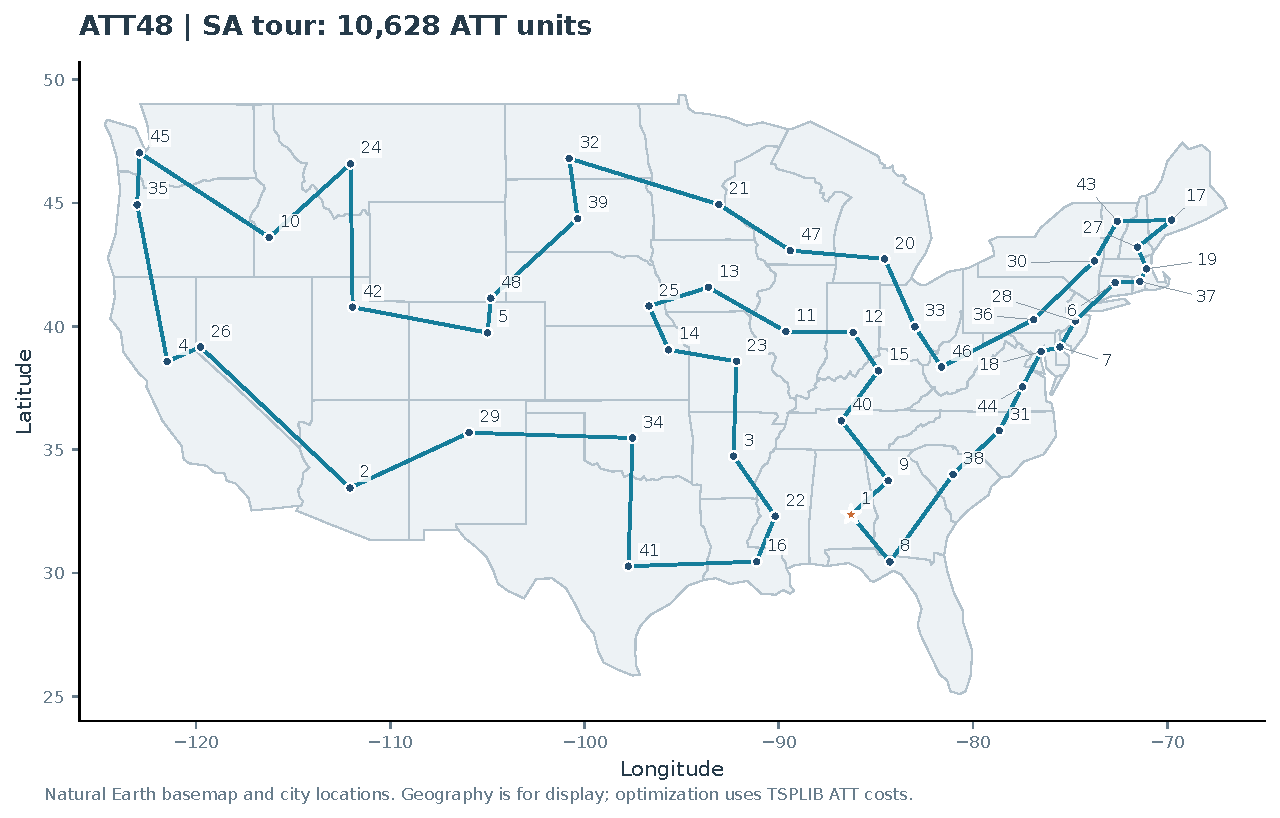
\includegraphics[width=.98\linewidth]{figures/att48_solution.pdf}
 \caption{种子 42 得到的最好闭环在地理地图上的展示，费用为 10628 ATT 单位，
 与官方最优值相同。橙色星形为节点 1（Alabama 州 Montgomery 首府），
 连线表示访问关系，并非实际道路。返回节点 1 的边已计入费用。}
 \label{fig:att-solution}
\end{figure}

完整访问顺序如下；按行连接，最后一个 1 表示返回起点：
\lstinputlisting[basicstyle=\ttfamily\small]{results/att48/route.txt}

\clearpage
\subsection{收敛过程与重复实验}
\cref{fig:att-convergence}展示种子 42 的费用变化。浅色曲线为每个温度层结束时的当前费用，
蓝色阶梯线为同一时刻的历史最好费用，虚线为公开最优值。
前期高温允许接受变差，当前费用存在明显起伏；随着温度降低，当前路线逐渐接近
历史最好路线。后者按定义单调不增。记录文件保存初始状态及全部 456 个温度层的末状态，
因此图中曲线是 457 个采样点；\textbf{这与实时窗口逐提案重绘的频率不同}。
首次最优解的提案编号由求解器单独记录，未由曲线采样位置估计。

\begin{figure}[htbp]
 \centering
 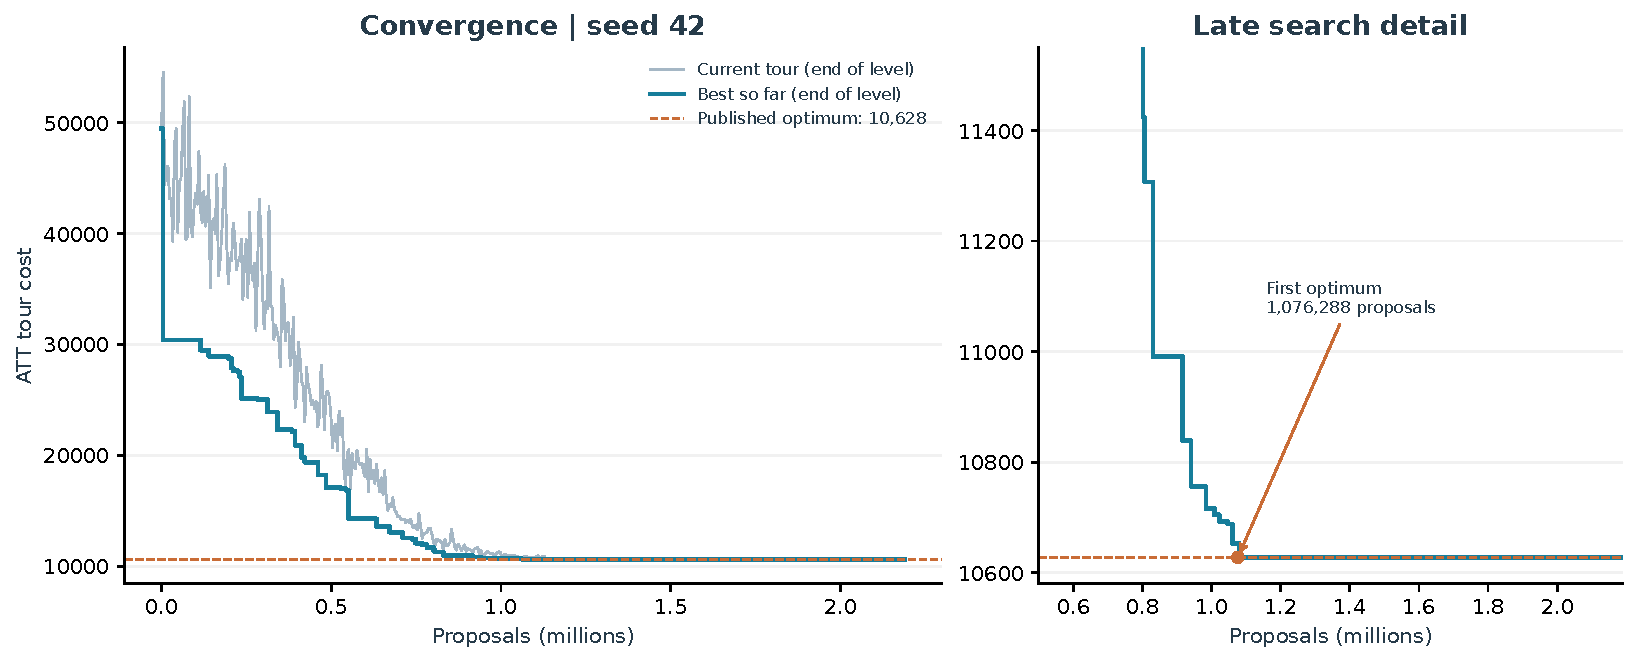
\includegraphics[width=\linewidth]{figures/att48_convergence.pdf}
 \caption{ATT48 模拟退火的收敛曲线及后期放大图。横轴为提案次数（百万），
 纵轴为闭环总费用；拒绝的候选也计入提案数。}
 \label{fig:att-convergence}
\end{figure}

\begin{table}[htbp]
 \centering\small
 \caption{20 次独立运行的实测结果；费用均为 ATT 单位，标准差采用样本标准差}
 \label{tab:att-results}
 \begin{tabularx}{.95\linewidth}{@{}XrXr@{}}
 \toprule
 指标 & 数值 & 指标 & 数值\\
 \midrule
 最好费用 & \AttBest & 最差费用 & \AttWorst\\
 平均费用 & \AttMean & 中位数 & \AttMedian\\
 样本标准差 & \AttStd & 达到最优值 & \AttHits/20\\
 平均相对差距 & \AttMeanGap\% & 平均单次求解时间 & \AttMeanTime{} s\\
 \bottomrule
 \end{tabularx}
\end{table}
相对差距定义为 $100(C-10628)/10628$。求解计时从初始排列生成前开始，
覆盖初温标定、全部搜索和内存中的记录，不包括数据读取、文件输出、绘图与编译。
短时间测量会受本机调度影响，不能直接视为其他计算机的运行时间。
20 次运行中只有 3 次达到最优值，说明即使在同一实例和预算下，随机种子也会影响结果。

\begin{figure}[!htbp]
 \centering
 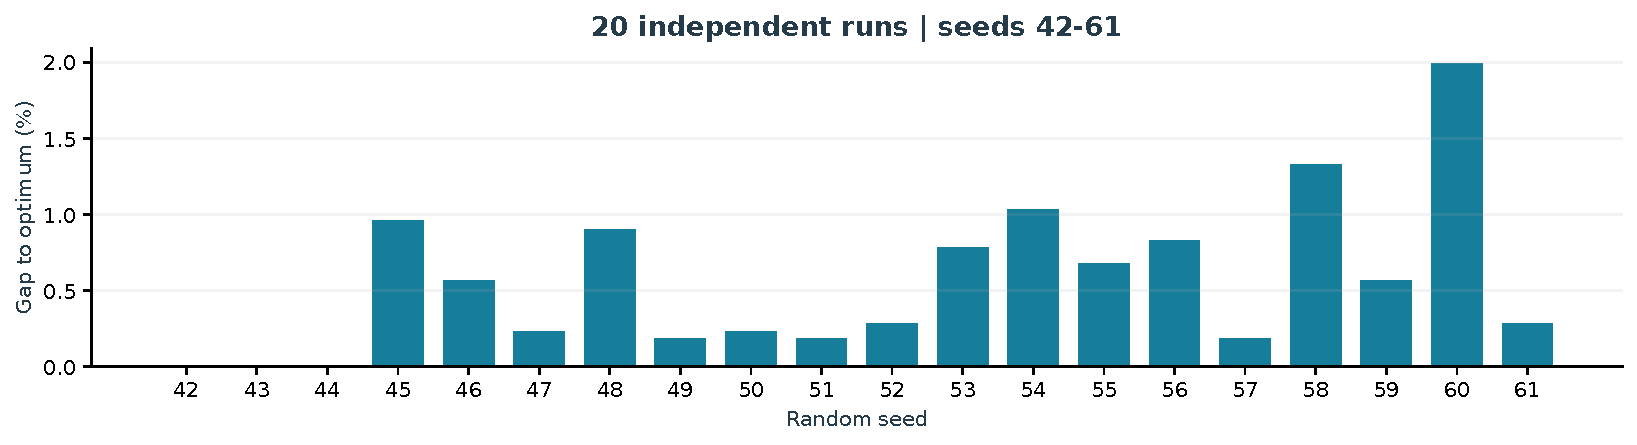
\includegraphics[width=.97\linewidth]{figures/att48_runs.pdf}
 \caption{连续种子 42--61 的最终费用相对于公开最优值的差距。零高度对应达到最优值。}
 \label{fig:att-runs}
\end{figure}

\clearpage
\subsection{复现命令与独立验证}
在项目根目录用 MinGW-w64 编译并运行。程序不带显示选项时，会在终端询问
\texttt{Visualize every proposal? [y/N]}；也可以通过选项直接决定：
\begin{lstlisting}[language=bash]
g++ -std=c++17 -O2 -static src/main.cpp -o build/tsp_sa.exe -lgdi32 -luser32
build/tsp_sa.exe --visual
build/tsp_sa.exe --no-visual --runs 20 --output results/att48
python scripts/verify_results.py
python scripts/make_figures.py
xelatex -output-directory=output/pdf tsp_simulated_annealing.tex
xelatex -output-directory=output/pdf tsp_simulated_annealing.tex
\end{lstlisting}
也可执行 \texttt{build.ps1} 自动创建编译目录。完整数据、图件和本节使用的结果已随项目保存，
无需重新联网即可编译文档；需要重绘时安装 \texttt{requirements-figures.txt} 中的依赖。
每个种子独立保存 \texttt{result.json}、\texttt{history.csv} 和 \texttt{best.tour}；
总目录的 \texttt{runs.csv} 汇总所有运行，\texttt{result.json} 保存这批运行中的最好结果。
本节数值宏与图件均由同一份结果文件自动生成。

\begin{figure}[htbp]
 \centering
 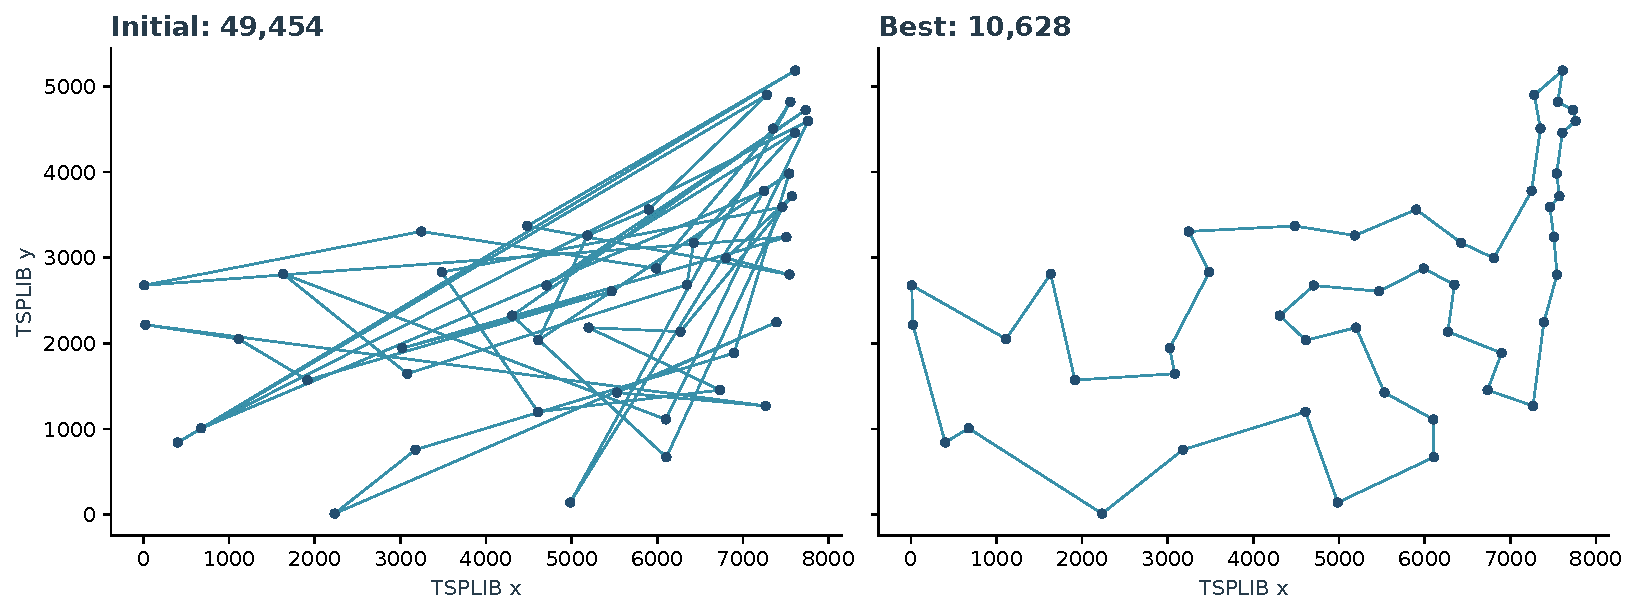
\includegraphics[width=\linewidth]{figures/att48_coordinate_tours.pdf}
 \caption{原始 TSPLIB 坐标系中的随机初始路线与求得的最好路线。
 本图直接使用求解坐标，不使用地理地图上的经纬度；两幅图采用相同尺度。}
 \label{fig:att-coordinates}
\end{figure}

\textbf{验证覆盖。}C++ 测试独立读取官方最优路线，按 ATT 规则重算得到 10628；
对 10 个随机排列中的全部位置对进行 10\,810 次四边增量与完整重算核对，包含返回起点边。
另检查小实例精确值、零距离、参数校验、固定种子复现、每次提案回调以及拒绝提案的刷新。
Windows 集成测试在真实窗口中验证暂停、单步及暂停状态下的三种关闭方式，
确认移除显示后仍完成全部提案，且路线和接受次数与无显示运行相同。
Python 校验脚本对全部 20 次实验逐一重算费用、检查完整排列、预算和收敛记录的单调性。


\clearpage
\begin{thebibliography}{9}
  \small
  \raggedright
  \setlength{\itemsep}{4pt}
  \bibitem{waterloo}
  University of Waterloo.
  \emph{The Traveling Salesman Problem: The Problem}.
  \url{https://www.math.uwaterloo.ca/tsp/problem/index.html}.

  \bibitem{cook}
  Cook, W.
  \emph{On the Solution of Traveling Salesman Problems}.
  \url{https://www.math.uwaterloo.ca/~bico/papers/tsp_icm.pdf}.

  \bibitem{kirkpatrick}
  Kirkpatrick, S., Gelatt, C. D., Jr., and Vecchi, M. P.
  Optimization by simulated annealing.
  \emph{Science}, 1983, 220(4598): 671--680.
  \href{https://doi.org/10.1126/science.220.4598.671}{doi:10.1126/science.220.4598.671}.

  \bibitem{metropolis}
  Metropolis, N., Rosenbluth, A. W., Rosenbluth, M. N., Teller, A. H., and Teller, E.
  Equation of state calculations by fast computing machines.
  \emph{The Journal of Chemical Physics}, 1953, 21(6): 1087--1092.
  \href{https://doi.org/10.1063/1.1699114}{doi:10.1063/1.1699114}.

  \bibitem{hajek}
  Hajek, B.
  Cooling schedules for optimal annealing.
  \emph{Mathematics of Operations Research}, 1988, 13(2): 311--329.
  \href{https://doi.org/10.1287/moor.13.2.311}{doi:10.1287/moor.13.2.311}.

  \bibitem{tsplib}
  Reinelt, G. \emph{TSPLIB 95: Documentation and TSP instances}.
  Universität Heidelberg.
  \url{https://comopt.ifi.uni-heidelberg.de/software/TSPLIB95/}.

  \bibitem{attbest}
  TSPLIB. \emph{Optimal solutions for symmetric TSPs: att48 = 10628}.
  \url{https://comopt.ifi.uni-heidelberg.de/software/TSPLIB95/tsp/TSP-BEST.html}.

  \bibitem{naturalearth}
  Natural Earth. \emph{Admin 1 -- States and Provinces (1:110m);
  Populated Places (1:10m)}. Public domain map data.
  \url{https://github.com/nvkelso/natural-earth-vector}.
\end{thebibliography}

\end{document}
